\section{Lists} % (fold)
\label{sec:lists}

\begin{frame}\frametitle{Lists}

    \begin{itemize}
        \item Group variables together
        \item Specific order
        \item Access items using square brackets: [ ]
    \end{itemize}

    However, do not confuse a list with the
    mathematical notion of a vector.

\end{frame}

\begin{frame}\frametitle{Accessing elements}\framesubtitle{The basics}

    \begin{itemize}
        \item First item: [0]
        \item Last item: [-1]
    \end{itemize}

    \codeblock{code/list_access.py}

    Note: can mix element types!

\end{frame}

\begin{frame}\frametitle{Slicing and adding}\framesubtitle{More on lists}

    \begin{itemize}
        \item Lists can be sliced: [2:5]
        \item Lists can be multiplied
        \item Lists can be added
    \end{itemize}

    % Look into this: confusing!
    \codeblock{code/list_add_slice.py}

\end{frame}

\begin{frame}\frametitle{Multiplication}\framesubtitle{Say what?}

    We can even multiply a list by an integer

    \codeblock{code/list_mult.py}

\end{frame}

\begin{frame}\frametitle{Lists are mutable}

    Lists are mutable, this means that individual elements can be changed.

    \codeblock{code/list_mutable.py}
    % list is unchanged after changing x

\end{frame}

\begin{frame}\frametitle{Copying a list}
    How to copy a list?

    % Look into this, confusing
    \codeblock{code/list_copy.py}.

\end{frame}

\begin{frame}\frametitle{What just happened?}
    Variables in Python really are tags:

    \begin{figure}
        \centering
        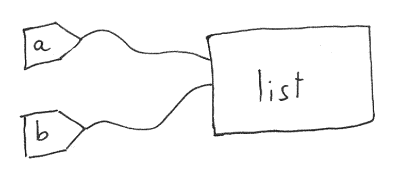
\includegraphics{img/list_tag.png}
    \end{figure}

    So \texttt{b = a} means: \texttt{b} is same tag as \texttt{a}.

    \vfill
    \tiny{Image from \url{http://henry.precheur.org/python/copy_list.html}}

\end{frame}

\begin{frame}\frametitle{Copying a list}

    Instead: we want:
    \begin{figure}
        \centering
        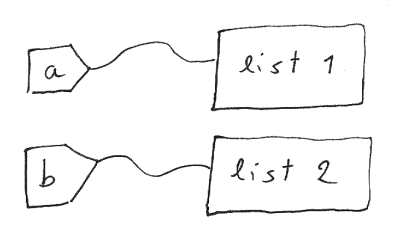
\includegraphics{img/list_tag2.png}
        \caption{\texttt{b = list(a)} or \texttt{b = a[:]}}
    \end{figure}

    \vfill
    \tiny{Image from \url{http://henry.precheur.org/python/copy_list.html}}

\end{frame}

\begin{frame}\frametitle{Copying a list}

    \codeblock{code/list_copy_id.py}

\end{frame}

\begin{frame}\frametitle{Functions modify lists}
    \framesubtitle{}

    Consider the following function:

    \codeblock{code/list_function.py}

    What is printed?

    \vfill \pause

    \texttt{[1, 2, 3]}, \texttt{[0, 2, 3]}

    \emph{Why does the list change, but variables do not?}

\end{frame}

\begin{frame}\frametitle{Why does the list change, but variables do not?}
    We have not changed the tag, only the contents of the list.
    The variable \texttt{l}, that is attached to the list, becomes local.
    The elements however, do not!

    \pause

    What happens in this case?
    \codeblock{code/list_function2.py}
\end{frame}

\begin{frame}\frametitle{More control over lists}

    \begin{itemize}
        \item \texttt{len(xs)}
        \item \texttt{xs.append(x)}
        \item \texttt{xs.count(x)}
        \item \texttt{xs.insert(i, x)}
        \item \texttt{xs.sort()} and \texttt{sorted(xs)}: what's the difference?
        \item \texttt{xs.remove(x)}
        \item \texttt{xs.pop()} or \texttt{xs.pop(i)}
        \item \texttt{x in xs}
    \end{itemize}

    \pause
    All these can be found in the Python documentation, google: `python list'

    Or using \texttt{dir(xs)} / \texttt{dir([])}

\end{frame}

\begin{frame}\frametitle{Looping over elements}

    It is very easy to loop over elements of a list using \texttt{for}, we have
    seen this before using \texttt{range}.

    \codeblock{code/list_loop.py}

\end{frame}

\begin{frame}\frametitle{Looping over elements}
\framesubtitle{and indices}
    Using \texttt{enumerate}, we can loop over both element and index at the same time.

    \codeblock{code/list_loop2.py}

\end{frame}

\begin{frame}\frametitle{Map}
    \framesubtitle{}

    We can apply a function to all elements of a list using \texttt{map}

    \codeblock{code/list_map.py}

\end{frame}

\begin{frame}\frametitle{Filter}
    \framesubtitle{}

    We can also filter elements of a list using \texttt{filter}

    \codeblock{code/list_filter.py}

\end{frame}

\begin{frame}\frametitle{List comprehensions}
    \framesubtitle{The powers of Python}

    A very powerful and concise way to create lists is using \emph{list comprehensions}

    \codeblock{code/list_compr_intr.py}

    This is often more readable than using \texttt{map} or \texttt{filter}

\end{frame}

\begin{frame}\frametitle{List comprehensions}\framesubtitle{Down the rabbit hole}

    \codeblock{code/list_compr.py}

    \pause

    Note how we can have a lists as elements of a list!

\end{frame}

\begin{frame}\frametitle{Implementing map using list comprehensions}

    Let's implement \texttt{map} using list comprehensions
    \pause

    \codeblock{code/list_mymap.py}

    Implement filter by yourself in one of the exercises.

\end{frame}

% section lists (end)
